\documentclass[11pt,a4paper]{article}
\usepackage{gtu-el-yazisi}
\begin{document}
\notbilgi{Elektronik I}{31.05 dersi -- Common-Base ve Common-Collector yükselteçler, MOSFET temelleri}{3105-elektronik-1.pdf}

\section{Common-Base Amplifier}
\noindent\sayfa{1}
\elcizimi[0.5]{sekiller/3105-elektronik-1-s1-1.png}[1]

\noindent\textbf{T model}
\begin{center}
\begin{circuitikz}[line width=0.6pt]
  \draw (2,4) -- (8.2,4) node[right]{$V_{out}$};
  \draw (4,4) node[circ]{} node[above]{$C$};
  \draw (2,4) to[cI, l=$\alpha i_e$] (2,2.4) node[circ]{} node[above left]{$B$} -- (1,2.4) node[ground]{};
  \draw (2,2.4) to[R, l_=$r_e$, i=$i_e$] (2,0.6) node[circ]{} node[left]{$E$};
  \draw (3.4,4) to[R, l=$r_o$] (3.4,0.6) -- (2,0.6);
  \draw[kursunkalem, line width=0.8pt] (2.6,0.2) -- (4.2,3.6);
  \draw (2,0.6) -- (2,-0.4) to[R, l=$R_{sig}$] (4.4,-0.4) to[sV, l=$v_{sig}$] (4.4,-1.8) node[ground]{};
  \node at (1.4,-0.8) {$\leftarrow R_{in}$};
  \draw (5.8,4) to[R, l=$R_C$] (5.8,2.4) node[ground]{};
  \draw (7.8,4) to[R, l=$R_L$] (7.8,2.4) node[ground]{};
  \draw[->] (6.8,2.4) node[below]{$R_{out}$} -- (6.8,3.7) -- (6.1,3.7);
\end{circuitikz}
\end{center}
\noindent
\begin{minipage}[c]{0.45\linewidth}
$V_A=\infty$\\
$r_o=\infty$
\end{minipage}\hfill
\begin{minipage}[c]{0.5\linewidth}
\centering
\fbox{$\begin{array}{l} R_{in}=r_e \\[1mm] R_{out}=R_C \end{array}$}
\[
  A_v=\ ?\ =\frac{v_{out}}{v_{sig}}
\]
\end{minipage}
\[
  \frac{v_{out}}{v_{sig}}=\frac{-\alpha\cdot i_e\,(R_C\,/\!/\,R_L)}{-i_e\,(R_{sig}+r_e)}
  =\frac{\alpha\,(R_C\,/\!/\,R_L)}{R_{sig}+r_e}
\]
$\Rightarrow$ if $R_{sig}\ll r_e$ \quad ignore $R_{sig}$\\
\hspace*{1cm}$\Rightarrow\ g_m\,(R_C\,/\!/\,R_L)$ \quad $\left[r_e=\dfrac{1}{g_m}\right]$

\sayfa{2}
\begin{itemize}[label=--]
  \item Small input Resistance \textcolor{kirmizikalem}{(opposite C-E)}\\
        \hspace*{1.5cm}$\nearrow$ normalde yüksek giriş direnci isteriz sinyalin zayıflamaması için
  \item Moderate -- High Output Resistance \textcolor{kirmizikalem}{(C-E)}
  \item High gain \textcolor{kirmizikalem}{(C-E)}
\end{itemize}

\section{Common-Collector Amplifier \textcolor{kirmizikalem}{(Emitter-Follower)}}
\elcizimi[0.65]{sekiller/3105-elektronik-1-s2-1.png}[2]

\noindent
\begin{minipage}[t]{0.45\linewidth}
\centering \underline{DC}
\elcizimi[0.35]{sekiller/3105-elektronik-1-s2-2.png}[2]
\end{minipage}\hfill
\begin{minipage}[t]{0.5\linewidth}
\centering \underline{AC} \qquad \textcolor{kirmizikalem}{\okunamadi{$A\neq\infty$}}
\elcizimi[0.5]{sekiller/3105-elektronik-1-s2-3.png}[2]
\end{minipage}

\noindent\sayfa{3}
\elcizimi[0.7]{sekiller/3105-elektronik-1-s3-1.png}[3]
\begin{align*}
  R_{in} &= \ ?\quad (R_{B1}\,/\!/\,R_{B2})\,/\!/\,\bigl(r_\pi+(\beta+1)(R_E\,/\!/\,R_L\,/\!/\,r_o)\bigr) \\
  R_{out} &= \ ?\quad r_o\,/\!/\,R_E\,/\!/\,\left(\frac{(R_{sig}\,/\!/\,R_{B1}\,/\!/\,R_{B2})+r_\pi}{\beta+1}\right)
\end{align*}
\[
  \textcolor{kirmizikalem}{\frac{V_{out}}{V_{sig}}}=\frac{V_\pi\,(g_m+1/r_\pi)\,R_L'}{V_\pi+V_\pi\,(g_m+1/r_\pi)\,R_L'}
  \qquad\Rightarrow\qquad
  \begin{array}{c}
    R_{sig}=0\ \text{(Assumption)} \\[1mm]
    V_{sig}=V_\pi+V_\pi\,(g_m+1/r_\pi)\,R_L'
  \end{array}
\]
\[
  A_v=\frac{V_{out}}{V_{sig}}=\frac{(g_m+1/r_\pi)\,R_L'}{1+(g_m+1/r_\pi)\,R_L'}
\]

\noindent Her zaman
\begin{itemize}[label=--]
  \item Voltage gain $<1$ \quad $(0{,}6\sim 0{,}\okunamadi{7})$
  \item High $\overset{\text{current}}{\text{output}}$ gain
  \item Input High Resistance
  \item Low Output resistance
\end{itemize}
You can use as\\
\hspace*{5mm}Voltage buffer
\begin{itemize}[label=--]
  \item Use it at the last stage of ripple stage amplifier
\end{itemize}
\begin{center}
\begin{circuitikz}[line width=0.6pt]
  \draw (0,0) node[ground]{} to[sV, l=$V_{sig}$] (0,1.5) -- (1,1.5);
  \draw (1,1.2) rectangle (2.4,1.8); \node[above] at (1.7,1.8) {$A_v>100$};
  \draw (2.4,1.5) -- (3.2,1.5);
  \draw (3.2,1.2) rectangle (4.6,1.8); \node[above] at (3.9,1.8) {$A_v\;50$};
  \draw (4.6,1.5) -- (5.4,1.5);
  \draw (5.4,1.2) rectangle (6.8,1.8); \node[above, align=center] at (6.1,1.8) {$A_v\approx 1$\\ \okunamadi{$(A_I\Rightarrow)$}};
  \draw (6.8,1.5) -- (8,1.5) to[R, l=$10\,\Omega$] (8,0) node[ground]{};
\end{circuitikz}
\end{center}

\section{Mosfet}
\noindent\sayfa{4}
\elcizimi[0.7]{sekiller/3105-elektronik-1-s4-1.png}[4]

\hfill Drain is positive

\subsection{5.1.3 Creating a channel for current Flow}
\elcizimi[0.4]{sekiller/3105-elektronik-1-s4-2.png}[4]

\textcolor{kirmizikalem}{$\vdots$}\\
Threshold Voltage ($V_T$) -- is the min value of $v_{GS}$

field effect!

\sayfa{5}
\noindent effective / overdrive voltage
\[
  v_{OV}=v_{GS}-V_t
\]
oxide capacitance ($C_{ox}$)
\[
  C_{ox}=\frac{\varepsilon_{ox}}{t_{ox}}\ \ \text{in F/m}^2 \qquad\qquad C=\frac{\varepsilon A}{d}
\]
\[
  |Q|=C_{ox}\,(WL)\,v_{OV}\ \ \text{in C}
\]

\subsection{Applying a small $v_{DS}$}
\[
  i_D=\left(C_{ox}\,W\,v_{OV}\right)\left(\frac{\mu_n\,v_{DS}}{L}\right)\ \text{A}
  \qquad \text{\small ? kontrol et}
\]
\textcolor{kursunkalem}{$\vdots$}\\
Small $v_{DS}$
\begin{align*}
  \text{(eq 5.7)}\quad i_D &= \left[(\mu_nC_{ox})\,\frac{W}{L}\,v_{OV}\right]v_{DS}\ \ \text{in A} \\
  \text{(eq 5.8a)}\quad r_{DS} &= \frac{v_{DS}}{i_D}=\frac{1}{(\mu_nC_{ox})\left(\frac{W}{L}\right)}\ \cdots
\end{align*}

\subsection{Operation as $v_{DS}$ increased}
\[
  v_{GD}=v_{GS}-v_{DS}
\]
$\rightarrow v$ \dots

\noindent\sayfa{6}
\elcizimi[0.5]{sekiller/3105-elektronik-1-s6-1.png}[6]

\noindent\textcolor{kirmizikalem}{$\bigstar$}\quad \textbf{Saturation Current formula}
\[
  I_D=\frac{1}{2}\,\underbrace{\overbrace{\mu_n\,C_{ox}}^{k_n'}\,\frac{W}{L}}_{k_n}\,(V_{GS}-V_t)^2
\]
\formulkutu{I_D=\mu_n\,C_{ox}\,\frac{W}{L}\left((V_{GS}-V_t)-\frac{1}{2}V_{DS}\right)V_{DS}}
\begin{center}
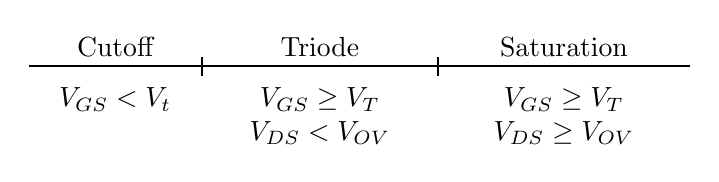
\begin{tikzpicture}[line width=0.6pt]
  \draw (0,0) -- (8.4,0);
  \foreach \x in {2.2,5.2} \draw (\x,-0.12) -- (\x,0.12);
  \node[above] at (1.1,0) {Cutoff};
  \node[above] at (3.7,0) {Triode};
  \node[above] at (6.8,0) {Saturation};
  \node[below] at (1.1,-0.15) {$V_{GS}<V_t$};
  \node[below, align=center] at (3.7,-0.15) {$V_{GS}\geq V_T$\\ $V_{DS}<V_{OV}$};
  \node[below, align=center] at (6.8,-0.15) {$V_{GS}\geq V_T$\\ $V_{DS}\geq V_{OV}$};
\end{tikzpicture}
\end{center}

\subsection{Operation for $v_{DS}\gg V_{OV}$}
\textcolor{kursunkalem}{$\vdots$}

\subsection{The p Channel MOSFET}
\[
  V_{SG}\geq |V_{tp}| \ \rightarrow\ V_{tp}<0
\]
\[
  V_{SG}<|V_t| \ \rightarrow\ \text{Cutoff}
\]

\sayfa{7}
\begin{center}
\begin{tabular}{lll}
  \toprule
  $V_{SG}\geq |V_T|$ & $\Rightarrow$ & \multirow{2}{*}{Saturation} \\
  $V_{SD}\geq V_{OV}$ & $\Rightarrow$ & \\ \midrule
  $V_{SG}\geq |V_t|$ & \multirow{2}{*}{$\Big\}$} & \multirow{2}{*}{\underline{Triode}} \\
  $V_{SD}<V_{OV}$ & & \\
\end{tabular}
\end{center}
\begin{align*}
  \text{(NMOS)}\quad I_{D1} &= \tfrac{1}{2}\,\mu_n\,C_{ox}\,\frac{W}{L}\,(V_{OV})^2 \\
  \text{(PMOS)}\quad I_{D2} &= \tfrac{1}{2}\,\mu_p\,C_{ox}\,\frac{W}{L}\,(V_{OV})^2
\end{align*}
if $\dfrac{W}{L}$, $C_{ox}$, $V_{OV}$ are equal $\Rightarrow$ $I_{D1}>I_{D2}$ because
\[
  \underset{\substack{\uparrow\\ \text{electron}\\ \text{mobility}}}{\mu_n}>\mu_p
\]

\section{Quick Recap}
The $i_D$--$v_{GS}$ Characteristics:\\
\hspace*{5mm}In sat

\begin{ornek}[(Ex 5.3)]
  \begin{align*}
    & I_D=0{,}4\ \text{mA} \\
    & V_D=0{,}5\ \text{V} \\
    & \mu_nC_{ox}=100\ \mu\text{A/V}^2 \qquad L=1\ \mu\text{m},\ W=32\ \mu\text{m}
  \end{align*}
  \[
    0{,}4\ \text{mA}=\frac{1}{2}\ 0{,}1\ \text{mA}\left(\frac{\overset{16}{\rlap{$\diagup$}32}}{1}\right)(V_{ov})^2
  \]
  \[
    V_{ov}=0{,}5 \ \leftarrow\ (V_{ov})^2=0{,}25 \ \rightarrow\ V_{ov}=+0{,}5
  \]
\end{ornek}

\sayfa{8}
\[
  V_{GS}=0{,}5+\overset{\curvearrowright\,V_T}{0{,}7} \qquad\qquad V_S=-1{,}2
\]
$R_S=$\\
\hspace*{5mm}$\vdots$

\begin{ornek}[(Ex 5.5)]
  \begin{align*}
    & V_{GS}\geq V_t & & V_{DS}\geq V_{ov} \\
    & 5-0\geq 1\ \text{V}\ \checkmark & & 0{,}1\geq 4\ \text{V}\ ?\ \times\ \ \text{Triode}
  \end{align*}
  \[
    I_D=\mu_nC_{ox}\,\frac{W}{L}\left(V_{ov}-\frac{1}{2}V_{DS}\right)V_{DS}
    \qquad\qquad r_{DS}=\frac{V_{DS}}{I_D}
  \]
  \[
    \hookrightarrow\ 1\ \text{mA/V}^2\,(4-0{,}05)\,0{,}1
  \]
  \[
    \kutula{I_D=0{,}395\ \text{mA}} \qquad\qquad \kutula{\frac{V_{DS}}{I_D}=253\ \Omega}
  \]
\end{ornek}

\begin{ornek}
\begin{minipage}[c]{0.5\linewidth}
\centering
\begin{circuitikz}[line width=0.6pt]
  \draw (0,0) node[nmos](M){};
  \draw (M.D) -- ++(0,0.3) to[R, l_=$1\,\text{k}$] ++(0,1.8) coordinate(T);
  \draw (M.G) -- ++(-1,0) coordinate(GG) to[R, l=$500\,\text{k}\Omega$] (GG |- T) -- (T);
  \path (GG |- T) -- (T) node[midway, above]{$5$ V};
  \draw (M.S) to[R, l=$2\,\text{k}$] ++(0,-1.6) node[ground]{};
  \node[text=kirmizikalem, align=left, below left] at (M.G) {$I_G=0$\\ $V_G=5$ V};
  \draw[->] (1.6,2.4) -- (1.6,-2.2);
\end{circuitikz}
\end{minipage}\hfill
\begin{minipage}[c]{0.45\linewidth}
  \begin{align*}
    & \mu_nC_{ox}\,\frac{W}{L}=0{,}25\ \text{mA/V}^2 \\
    & V_{tn}=2\ \text{V} \\
    & \lambda=0 \qquad V_A=\okunamadi{0\,\text{V}} \\
    & I_D,\ V_G,\ V_S,\ V_D=\ ?
  \end{align*}
\end{minipage}
\end{ornek}

\sayfa{9}
\begin{align*}
  I_D &= \frac{1}{2}\,\mu_nC_{ox}\,\frac{W}{L}\,(V_{GS}-V_t)^2 \\
  I_D &= \frac{1}{2}\ 0{,}25\ \text{mA/V}^2\,(5-V_S-2)^2 \\
  I_D &= \frac{1}{2}\ 0{,}25\ \text{mA/V}^2\,(3-V_S)^2 \\
  I_D &= \frac{1}{2}\ \frac{0{,}25\ \text{mA}}{\text{V}^2}\,(3-2I_D)^2 \\
  I_D &= \frac{1}{2}\ \frac{0{,}25\ \text{mA}}{\text{V}^2}\left(9+4I_D^2-6I_D\right) \qquad\text{\footnotemark} \\
  8I_D &= 9+4I_D^2-6I_D \\
  & \qquad\qquad 4I_D^2-14I_D+9=0
\end{align*}
\footnotetext{Claude notu: muhtemelen $(3-2I_D)^2=9+4I_D^2-12I_D$ olmalı; bu durumda denklem $4I_D^2-20I_D+9=0$ olur.}

\end{document}
